% Compile with: xelatex report.tex   (NOT pdflatex -- needs xeCJK for Chinese)
\documentclass[11pt]{article}
\usepackage[a4paper,margin=1in]{geometry}
\usepackage{graphicx}
\usepackage{amsmath}
\usepackage{listings}
\usepackage{xcolor}
\usepackage{booktabs}
\usepackage{hyperref}
\usepackage{xeCJK}
\setCJKmainfont{PingFang TC}
\usepackage{float}

\lstset{
  basicstyle=\ttfamily\small,
  breaklines=true,
  columns=fullflexible,
  keepspaces=true,
  frame=single,
  framesep=4pt,
  rulecolor=\color{black!30},
  backgroundcolor=\color{black!3},
}

\title{HW4 -- Traveling Salesperson Problem\\[2pt]\large Branch and Bound}
\author{Student ID: \texttt{112000112 , 112080008} \quad Name: \texttt{施又歆 , 黃品瑄}}

\begin{document}
\maketitle

\section{Pseudocode of the Branch-and-Bound Algorithm}

\subsection*{Lower bound}

For every city $i$, let $\mathit{minOut}[i]=\min_{j \ne i} C[i][j]$.
Any complete tour must use exactly one outgoing edge from each city, so the
cost of any tour is at least $\sum_i \mathit{minOut}[i]$.  When the search has
fixed a partial path $v_0,v_1,\dots,v_{d-1}$ with
$\mathit{current}=v_{d-1}$, the outgoing edges of $v_0,\dots,v_{d-2}$ are
already chosen (their cost is already in $\mathit{cost}$), but the outgoing
edges of $\mathit{current}$ and of every unvisited city are not yet
determined.  Hence the remaining cost is at least
\[
\mathit{remMin} \;=\; \mathit{minOut}[\mathit{current}]
                     \;+\; \sum_{u \notin \text{visited}} \mathit{minOut}[u].
\]
$\mathit{remMin}$ is maintained incrementally: when the algorithm extends the
path with an edge from $\mathit{current}$ to $\mathit{next}$,
$\mathit{current}$'s outgoing edge becomes fixed, so
$\mathit{remMin}' = \mathit{remMin} - \mathit{minOut}[\mathit{current}]$.

\subsection*{Pseudocode}

\begin{lstlisting}
Algorithm  TSP-BranchAndBound(C, n)
Input :    n x n cost matrix  C
Output:    A shortest Hamiltonian cycle starting and ending at city 1,
           and its total cost.

  /* ---------- 1. Pre-computation ---------- */
  for i = 1 to n
      minOut[i] <- min_{j != i} C[i][j]
  totalMin   <- sum_{i=1..n} minOut[i]

  /* ---------- 2. Initial upper bound (nearest neighbour) ---------- */
  visited[1]   <- true,  visited[2..n] <- false
  cur          <- 1,  cost <- 0,  path <- (1)
  for k = 2 to n
      pick the unvisited city  j  with smallest  C[cur][j]
      append j to path,  visited[j] <- true
      cost <- cost + C[cur][j];   cur <- j
  bestCost <- cost + C[cur][1]
  bestPath <- path

  /* ---------- 3. Depth-first branch and bound ---------- */
  visited[1] <- true,  curPath <- (1)
  DFS(1, 1, 0, totalMin)

  output bestPath, bestCost


Procedure  DFS(current, depth, cost, remMin)

  /* base case: every city has been placed */
  if depth = n then
      total <- cost + C[current][1]
      if total < bestCost then
          bestCost <- total;  bestPath <- curPath
      return

  /* current's outgoing edge is about to be chosen, so it leaves remMin */
  newRemMin <- remMin - minOut[current]

  /* expand the children sorted by edge cost (best-first) */
  cand <- empty list
  for next = 1 to n
      if not visited[next] then
          append (C[current][next], next) to cand
  sort cand in ascending order of the first coordinate

  for each (edge, next) in cand
      newCost <- cost + edge
      /* PRUNE: best achievable from this branch is newCost + newRemMin  */
      if newCost + newRemMin >= bestCost then
          break        /* later candidates are worse, so cut them all     */
      visited[next]   <- true
      append next to curPath
      DFS(next, depth + 1, newCost, newRemMin)
      remove last element of curPath
      visited[next]   <- false
\end{lstlisting}

\subsection*{Correctness and Complexity}
\begin{itemize}
  \item \textbf{Correctness.} $\mathit{cost} + \mathit{remMin}$ is a valid
        lower bound on the cost of any completion of the current partial
        tour, because each remaining outgoing edge contributes at least its
        row-minimum.  Pruning a subtree whose lower bound is at least
        $\mathit{bestCost}$ therefore cannot discard the optimum.  An
        initial upper bound is obtained from a feasible nearest-neighbour
        tour.
  \item \textbf{Worst-case complexity.} $O(n!)$ -- the same as exhaustive
        search.  In practice the bound and the nearest-neighbour seed prune
        the vast majority of branches, giving the running times reported
        below.
\end{itemize}

\section{Running-time Comparison}

\subsection*{Raw timings (seconds)}

\begin{center}
\scriptsize
\setlength{\tabcolsep}{4pt}
\begin{tabular}{r ccccc cc}
\toprule
    & \multicolumn{5}{c}{Branch \& Bound (seconds)} & \multicolumn{2}{c}{Brute Force (seconds)} \\
\cmidrule(lr){2-6}\cmidrule(lr){7-8}
$n$ & Data 1 & Data 2 & Data 3 & avg & $\log_{10}$avg & Data 1 & $\log_{10}$time \\
\midrule
 5 & 0.000007 & 0.000004 & 0.000003 & 0.000005 & $-5.331$ & 0.000016    & $-4.796$ \\
 6 & 0.000007 & 0.000003 & 0.000007 & 0.000006 & $-5.247$ & 0.000008    & $-5.097$ \\
 7 & 0.000009 & 0.000005 & 0.000007 & 0.000007 & $-5.155$ & 0.000020    & $-4.699$ \\
 8 & 0.000022 & 0.000012 & 0.000001 & 0.000012 & $-4.933$ & 0.000094    & $-4.027$ \\
 9 & 0.000080 & 0.000012 & 0.000055 & 0.000049 & $-4.310$ & 0.000654    & $-3.184$ \\
10 & 0.000083 & 0.000192 & 0.000015 & 0.000097 & $-4.014$ & 0.005374    & $-2.270$ \\
11 & 0.000066 & 0.000185 & 0.000329 & 0.000193 & $-3.714$ & 0.053291    & $-1.273$ \\
12 & 0.000261 & 0.000094 & 0.000301 & 0.000219 & $-3.660$ & 0.620553    & $-0.207$ \\
13 & 0.000331 & 0.001015 & 0.000601 & 0.000649 & $-3.188$ & 7.786247    & $\phantom{-}0.891$ \\
14 & 0.001949 & 0.003494 & 0.001850 & 0.002431 & $-2.614$ & 106.276025  & $\phantom{-}2.026$ \\
15 & 0.006952 & 0.028169 & 0.006962 & 0.014028 & $-1.853$ & --- (> 180) & --- \\
16 & 0.000876 & 0.001260 & 0.031666 & 0.011267 & $-1.948$ & --- (> 180) & --- \\
\bottomrule
\end{tabular}
\end{center}

\subsection*{Plots}

\begin{figure}[H]
\centering
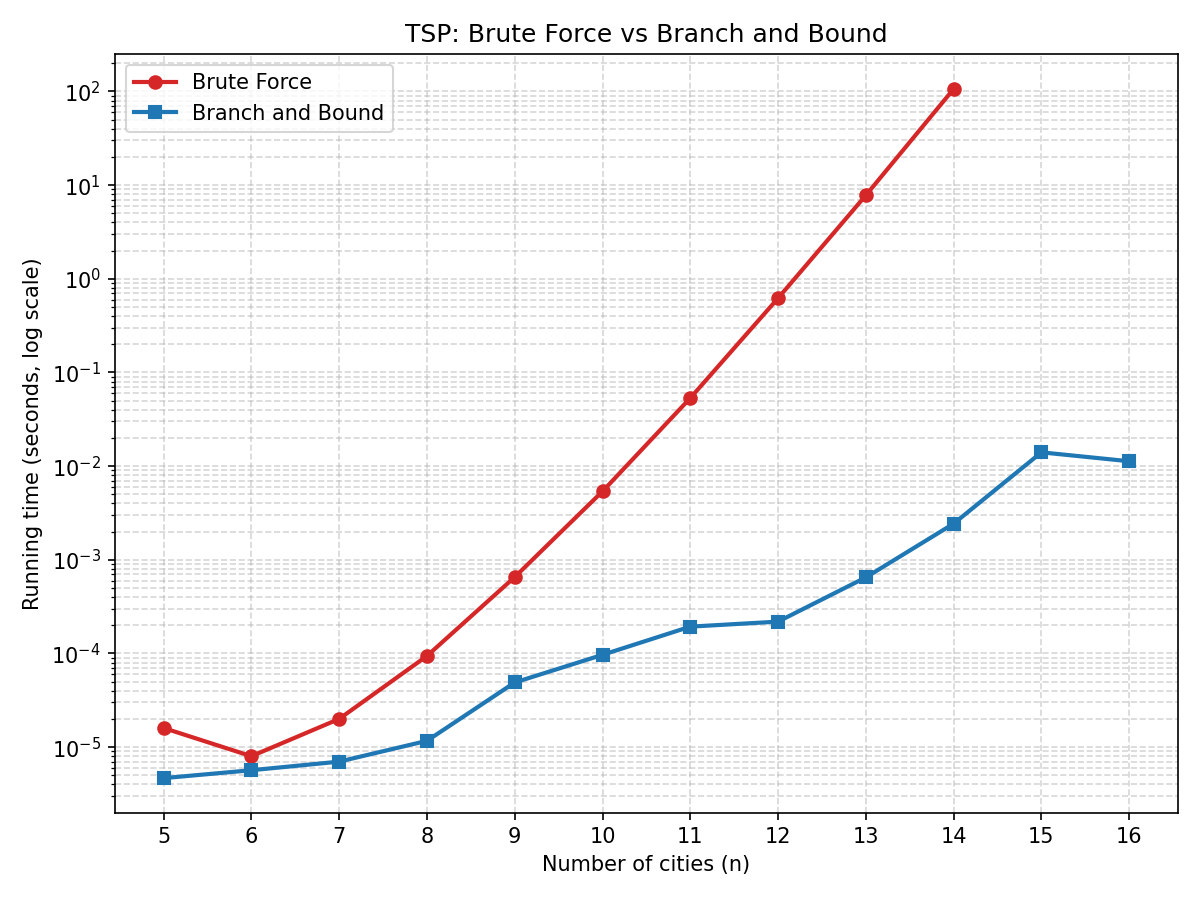
\includegraphics[width=0.85\linewidth]{timing_plot.png}
\caption{Running time on a logarithmic y-axis (seconds).}
\end{figure}

\begin{figure}[H]
\centering
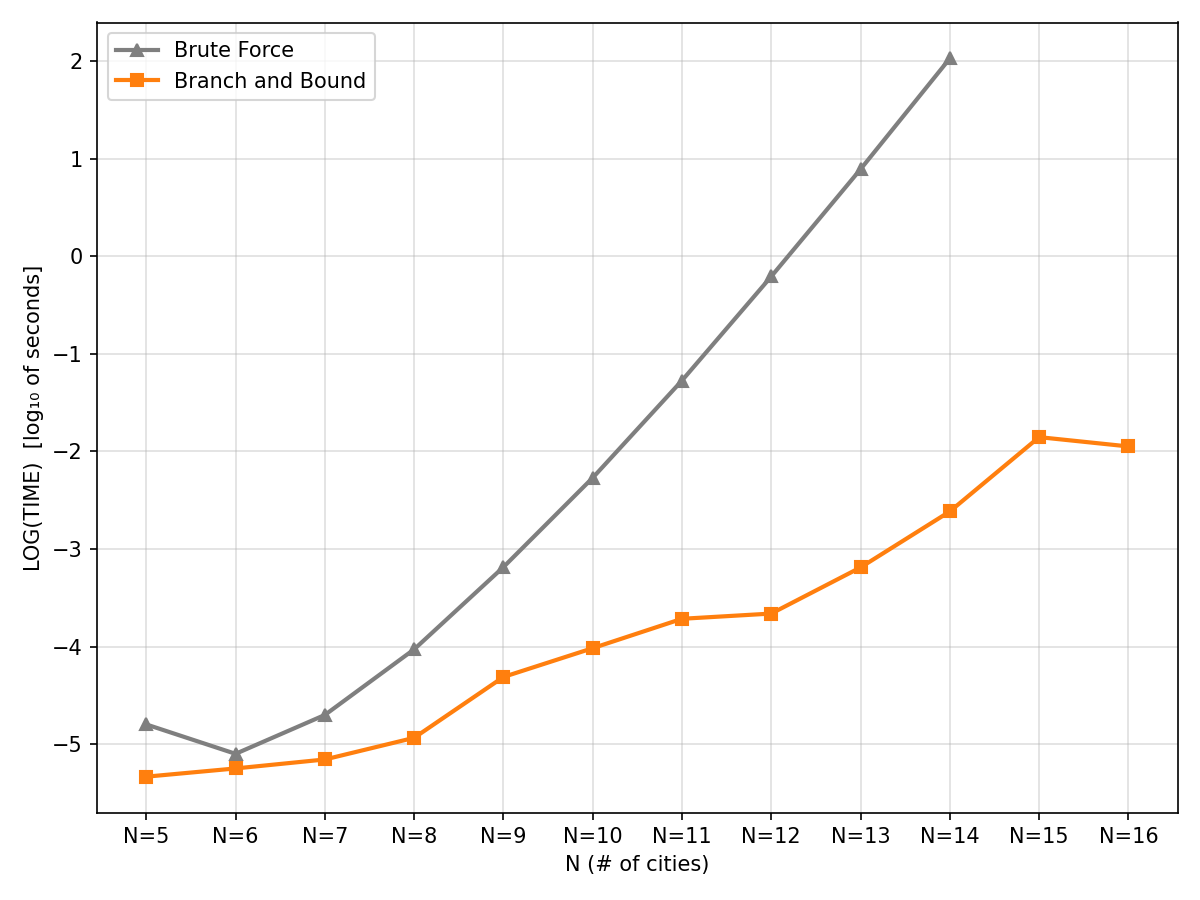
\includegraphics[width=0.85\linewidth]{timing_plot_log.png}
\end{figure}

n = 15 and n = 16 are predicted more than 25 min and 6 hours respectively, so they are not shown in the graph.

\paragraph{Hardware / software.}
Local benchmark machine: MacBook (Mac15,12) with Apple~M3 CPU, 24~GB RAM,
macOS~14.5.  Compiler: Apple~clang~15.0 invoked as
\texttt{g++ -std=c++11 -O2}. 
\end{document}
